% !TEX root = ../main.tex
% Chapter 2 --- Background

\chapter{Background}\label{ch:background}

This chapter covers the two foundations the rest of the work rests on: the neural-process
architecture and what its predictive distribution can say (\sref{sec:bg-neural-processes}), and why
the atmospheric state rather than the coarse surface field should drive it
(\sref{sec:bg-atmos-vs-surface}).

\section{Neural Processes for Downscaling}\label{sec:bg-neural-processes}

Neural processes were introduced to address some of the shortcomings of Gaussian processes: they still return a predictive distribution, while dropping the cubic cost of exact conditioning and the need to choose a kernel by hand~\cite{garnelo2018cnp}. The family was in a second step extended with translation equivariance so that it could be applied to spatial fields~\cite{gordon2020convcnp}.

A conditional neural process reads a set of context observations and returns a predictive distribution at any target coordinate, in one forward pass and without conditioning on a kernel~\cite{garnelo2018cnp}. The distribution it returns is whatever its output head parameterises, so the same backbone can serve a Gaussian for temperature and a Bernoulli--Gamma for precipitation. What the original CNPs lose is geometry: they squeeze the context set into a single fixed-length vector, so where an observation sat relative to its neighbours is gone by the time the decoder sees it. Convolutional CNPs keep it by mapping the context onto a function over space and refining that with a CNN, which also makes the model translation equivariant~\cite{gordon2020convcnp}.

The predictive distribution factorises into per-point marginals: a ConvCNP is calibrated at each target point but says nothing about how the error at one point relates to its neighbour, so independent draws do not form a coherent field. This belongs to the output head rather than to the family: a joint Gaussian head~\cite{andersson2023convgnp} or autoregressive sampling from a trained model~\cite{bruinsma2023arcnp} would recover the dependence. Neither is used here; both models in this work keep the factorised head.
\section{The Potential of Atmospheric Input}\label{sec:bg-atmos-vs-surface}



Weather in mountainous terrain is shaped by local effects that global models resolve only poorly. In Switzerland, the most prominent examples are Foehn in the inner Alpine valleys and afternoon convection over the Prealpine foothills. Part of the problem is simply the resolution of the driving field and whether it resolves the local terrain at all (\sref{sec:intro-motivation}).



The other part of the problem is that meteorological processes are mainly driven by the atmosphere. The surface is easy to measure, but what it shows is largely a response to the atmosphere above it, which is harder to observe yet carries the information that actually drives the weather. Direct measurements of the vertical structure come from radiosoundings, launched twice a day from Payerne alone, and from the ascent and descent profiles of commercial aircraft~\cite{meteoswiss_aircraft}. Neither is dense enough to drive a downscaling model, which is why the atmospheric state has to come from a reanalysis or a forecast model.



One example for research on these complex relations in a different context than downscaling is \textcite{panziera2010}, who analysed orographic precipitation events on the southern side of the Swiss Alps and found the rainfall pattern best explained by the mesoscale wind in specific layers aloft, together with the stability of the incoming air mass: a case where the surface field carries the consequence of an atmospheric process rather than its cause.



A classical way to look at that vertical information is a thermodynamic diagram such as an emagram, which plots the temperature and dew-point profiles of a sounding against reference lines for dry and moist adiabats. Often it also includes wind direction and strength. This representation is heavily used by meteorologists, for aviation forecasts as well as for weather estimation in sports such as paragliding. They provide much information at a single glance: how stable the atmosphere is, at what altitude convective clouds will form, and how much convective energy is available. \fref{fig:emagram-payerne} shows a visualisation of such an emagram using atmospheric data for Payerne, the Swiss radiosounding station. 



\begin{figure}[H]

\centering

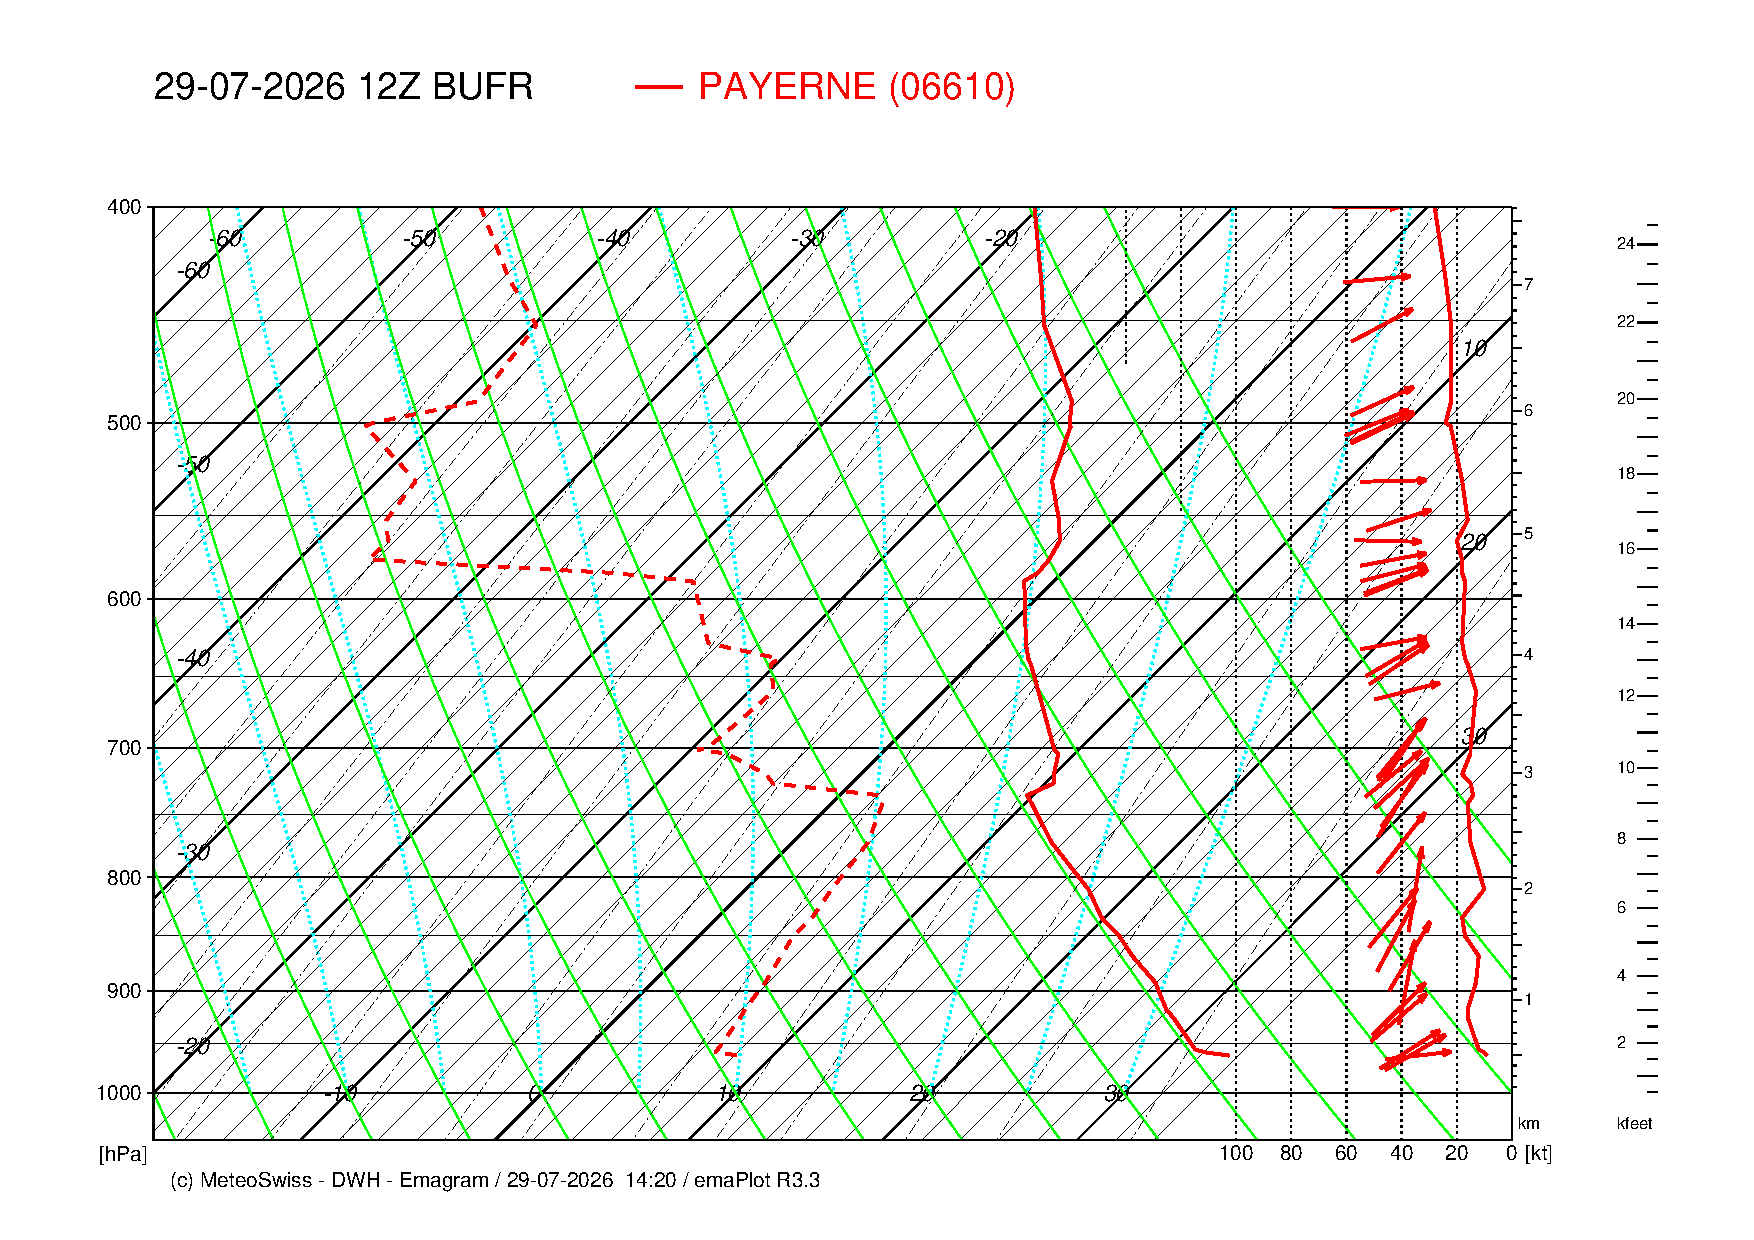
\includegraphics[width=0.8\textwidth]{images/radio-soundings_emagram_payerne.20260729_1200.pdf}

\caption[Emagram of the Payerne radiosounding]{Emagram of the radiosounding at Payerne (station 06610) on 29 July 2026, 12~UTC. Temperature and dew point are plotted against pressure, with the wind profile on the right and height given in both km and kfeet. Copy from MeteoSwiss~\cite{meteoswiss_radiosounding}.}

\label{fig:emagram-payerne}

\end{figure}



Alpine weather and specifically precipitation is also strongly seasonal and diurnal: winter events are predominantly frontal, whereas summer events are largely convective and peak in the afternoon~\cite{nisi2020}. On a typical summer day, a stable layer caps the boundary layer in the morning and suppresses convection. As the sun gradually heats the ground, this stable layer is resolvced. Once it breaks, thermals develop and the convective boundary layer expands to roughly \SIrange{2}{3}{km}; where sufficient convective energy is available, the resulting cumulus clouds grow far beyond that and produce thunderstorms. Whether the cap breaks at all depends on its strength in competition with the heat supplied at the surface, which is why a single daily snapshot of the atmosphere is likely not enough to capture these events.



We aim here to develop a model that can learn the relevant weather processes, rather than provide just accurate predictions. To do that, we try to select a strategic set of input channels that enable the model to learn these relevant processes without the need of hourly data. We therefore include snapshots of the vertical structure of the atmosphere as input, in addition to or as a replacement for surface input. The vertical structure is available from the ERA5 reanalysis of \textcite{hersbach2020era5}, which provides a continuous representation of the atmosphere in the form of curves of temperature, humidity and wind speed against pressure levels\footnote{Low pressure levels represent high altitude layers and high pressure levels are close to the surface.}. These curves are available at every grid point and every hour. To capture the diurnal cycle of convective events, we sample the atmospheric channels at five times of day (00, 06, 12, 15 and 18~UTC), so that the model sees both the capped morning state and the state after the expected breakup, i.e.\ the daily evolution rather than only a daily mean.



Sampling through the day turns a static description of the atmosphere into one that possibly can describe the physical process. \textcite{vaughan2022convcnp} already combine atmospheric with surface channels, but they report neither the timing of those fields nor what each group of channels contributes; \sref{sec:meth-fi} sets out to measure that.

